\documentclass[10pt]{beamer}

%ADICIONADOS POR MIM
\usepackage[utf8]{inputenc}
\usepackage{datetime}
\usepackage{ragged2e}
\usepackage{wrapfig}
\usepackage{multirow}
\usepackage[most]{tcolorbox}
%

\usetheme[progressbar=frametitle]{metropolis}

\usepackage{booktabs}
\usepackage[scale=2]{ccicons}

\usepackage{pgfplots}
\usepgfplotslibrary{dateplot}

\usepackage{xspace}
%\apptocmd{\frame}{}{\justifying}{} % Allow optional arguments after frame.
\newcommand{\themename}{\textbf{\textsc{metropolis}}\xspace}

\title{Modelagem e Controle de Biorreatores Anaeróbicos}
%\subtitle{A modern beamer theme}
\date{Outubro de 2017}
\author{William Cechin Guarienti}
\institute{Prof. Orientador: Diego Eckhard}
%\institute{Center for modern beamer themes}
\titlegraphic{\hfill\includegraphics[height=1.5cm]{figures/logo}}

\begin{document}

\maketitle

\begin{frame}{Conteúdo da apresentação}
  \setbeamertemplate{section in toc}[sections numbered]
  \tableofcontents[hideallsubsections]
\end{frame}

\section{Objetivo}

\begin{frame}[fragile]{Objetivo}
\justifying
O objetivo do projeto de pesquisa é projetar um controlador para a regulação da vazão de gás metano em um biorreator, com o intuito de otimizar sua produção. 
%Tal estudo está no escopo do desenvolvimento de fontes de energia sustentáveis, pois um dos produtos gerados pelo biorreator é o gás metano. 
%Dessa forma, promove-se a sustentabilidade econômica, pois a utilização de biorreatores estimula o correto destino de dejetos industriais, que são processados para a formação de combustíveis e fertilizantes.
  
\end{frame}



\section{Metodologia}

\begin{frame}{Metodologia}
	Para que possamos compreender o funcionamento do biorreator anaeróbico e otimizar sua produção, precisamos:
	\begin{itemize}
		\item Determinarmos um modelo adequado para o estudo, com base no processo bioquímico que ocorre em seu interior;
		\item Estudar o(s) ponto(s) de equilíbrio do processo;
		\item Estimar o esforço de controle em RP necessário para produzir a vazão de gás desejada;
		\item Projetar um controlador PI para o processo.
	\end{itemize}
\end{frame}

\section{Desenvolvimento}

\subsection{Processo bioquímico}
\begin{frame}[fragile]{Processo bioquímico}
\begin{center}
\begin{figure}
\includegraphics[height=5cm]{figures/biorreator.png}
\caption{Biorreatores utilizados para a produção dos dados utilizados neste trabalho}
\end{figure}
\end{center}
\end{frame}

%\begin{frame}[fragile]{Processo bioquímico}
%\begin{center}
%\begin{figure}
%\includegraphics[height=7cm]{bioquimica.png}
%\caption{Representação simplificada do processo de degradação anaeróbica \cite{de2003methane}}
%\end{figure}
%\end{center}
%\end{frame}

\subsection{Determinação do modelo matemático}
\begin{frame}[fragile]{Determinação do modelo matemático}

\begin{columns}
\begin{column}{0.65\textwidth}
\begin{itemize}[<+- | alert@+>]
\item $\dot{x_{1}}(t)=[v_{1}(S_{1}(t))-p_7 \cdot D - p_8]\cdot x_1(t)$\\
\item $\dot{x_{2}}(t)=[v_{2}(S_{2}(t))-p_7 \cdot D - p_9]\cdot x_2(t)$\\
\item $\dot{S_{1}}(t)=D\cdot(S_{1}^{in} - S_{1}(t)) - p_{10} \cdot v_{1}(S_{1}(t))\cdot x_1(t)$\\
\item $\dot{S_{2}}(t)=D \cdot (S_{2}^{in} - S_{2}(t)) + p_{11}\cdot v_{1}(S_{1}(t)) \cdot x_1(t) - p_{12} \cdot v_{2}(S_{2}(t)) \cdot x_2(t) $\\
\item $\dot{C}(t)= p_{14} \cdot v_{1}(S_{1}(t)) \cdot {x_{1}}(t) + p_{16} \cdot v_{2}(S_{2}(t)) \cdot {x_{2}}(t) - p_{15} \cdot C(t) $\\
\end{itemize}

\vspace{10pt}
\begin{footnotesize}
$x_1(t)$: concentração de bactérias acinogênicas [mg/L]; \\
$x_2(t)$: concentração de bactérias metanogênicas [mg/L];\\
$S_1(t)$: concentração de substrato orgânico (COD) [mg/L];\\
$S_2(t)$: concentração dos ácidos graxos voláteis [mmol/L];\\
$C(t)$: concentração de carbono inorgânico (mmol/L)\\
$D$: taxa de diluição dos influentes;\\
$p_i$: constantes determinadas experimentalmente;\\
\end{footnotesize}
\end{column}

\begin{column}{0.35\textwidth} 
    \begin{center}
    \begin{figure}
    \includegraphics[width=1\textwidth]{figures/esquema_biorreator.png}
     \caption{Representação simplificada de um biorreator}
    \end{figure}
     \end{center}
\end{column}
\end{columns}

\end{frame}

\begin{frame}[fragile]{Determinação do modelo matemático}
\textbf{Lei de Haldane:}
\begin{equation*}
v_i = p_{3i-2}\frac{S_i(t)}{p_{3i-1}+S_i(t)+p_{3i}\cdot(S_i(t))^2}  \hspace{2cm} i=1,2
\end{equation*}
\vspace{20pt}
\begin{footnotesize}
$p_i$: coeficientes determinados experimentalmente;
\end{footnotesize}
    \begin{center}
    \begin{figure}[b]
    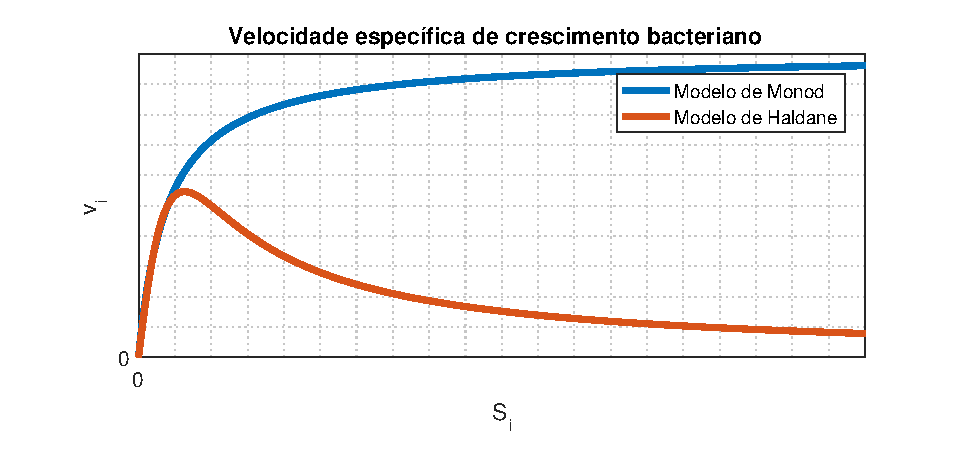
\includegraphics[width=.8\textwidth]{figures/velocidade.eps}	
     \caption{Representação da equação de Haldane}
    \end{figure}
     \end{center}
\end{frame}

\begin{frame}[fragile]{Determinação do modelo matemático}
Taxa de fluxo de gás na saída do biorreator $q(t)$:\\
\begin{equation*}
q(t) = p_{13}\cdot v_{2}(S_{2}(t))x_2(t) + p_{15}\cdot C(t)
\end{equation*}
\\
\begin{footnotesize}
$p_i$: coeficientes (constantes) determinados experimentalmente;
\end{footnotesize}

    \begin{center}
    \begin{figure}[b]
    \includegraphics[width=0.5\textwidth]{figures/coletores.png}+
     \caption{Coletores usados para medição do biogás \cite{eckhard}}
    \end{figure}
     \end{center}

\end{frame}

\subsection{Pontos de equilíbrio do processo}
\begin{frame}[fragile]{Pontos de equilíbrio do processo}
Dada uma referência $r$ constante, obtém-se numericamente $S_{1}^{in}$ e o(s) ponto(s) de equilíbrio do sistema utilizando métodos numéricos. Assume-se que a taxa de diluição ($D$) é constante e o vetor de parâmetros \textbf{p} é conhecido. 
\end{frame}

\begin{frame}[fragile]{Pontos de equilíbrio do processo}

\begin{columns}

\begin{column}{0.5\textwidth}
\begin{footnotesize}

\begin{table}[!b]
\centering
\begin{tabular}{l|l|l|}
\hline
\multicolumn{1}{|l|}{\multirow{2}{*}{$\dot{x_1}=0$}} & \multicolumn{2}{l|}{\multirow{2}{*}{\begin{tabular}[c]{@{}l@{}}$S_1$ depende apenas dos \\ parâmetros do biorreator\end{tabular}}} \\
\multicolumn{1}{|l|}{}                     & \multicolumn{2}{l|}{}                                                                                                              \\ \hline
\multicolumn{1}{|l|}{$\dot{x_2}=0$}                  & \multicolumn{2}{l|}{\begin{tabular}[c]{@{}l@{}}$S_2$ depende apenas dos \\ parâmetros do biorreator\end{tabular}}                  \\ \hline
                                           & Se...                                                                   & Então...                                                 \\ \hline
\multicolumn{1}{|l|}{$\dot{S_1}=0$}        & $S_{1}^{in} \uparrow$                                                   & $x_1 \uparrow$                                           \\ \hline
\multicolumn{1}{|l|}{$\dot{S_2}=0$}        & $x_1 \uparrow$                                                          & $x_2 \uparrow$                                           \\ \hline
\multicolumn{1}{|l|}{$\dot{C}=0$}          & $x_1 \uparrow \& x_2 \uparrow$                                          & $C \uparrow$                                             \\ \hline
\multicolumn{1}{|l|}{$q$}                & $x_2 \uparrow \& C \uparrow$                                            & $q \uparrow $                                          \\ \hline
\end{tabular}
\caption{\begin{footnotesize} Influência de $S_{1}^{in}$ nos estados (em equilíbrio)\end{footnotesize} }
\end{table}

\end{footnotesize}
\end{column}

\begin{column}{0.5\textwidth}
\begin{footnotesize}
\begin{itemize}[<+- | alert@+>]
\item $\dot{x_{1}}(t)=[v_{1}(S_{1}(t))-p_7 \cdot D - p_8]\cdot x_1(t)$\\
\item $\dot{x_{2}}(t)=[v_{2}(S_{2}(t))-p_7 \cdot D - p_9]\cdot x_2(t)$\\
\item $\dot{S_{1}}(t)=D\cdot(S_{1}^{in} - S_{1}(t)) - p_{10} \cdot v_{1}(S_{1}(t))\cdot x_1(t)$\\
\item $\dot{S_{2}}(t)=D \cdot (S_{2}^{in} - S_{2}(t)) + p_{11}\cdot v_{1}(S_{1}(t)) \cdot x_1(t) - p_{12} \cdot v_{2}(S_{2}(t)) \cdot x_2(t) $\\
\item $\dot{C}(t)= p_{14} \cdot v_{1}(S_{1}(t)) \cdot {x_{1}}(t) + p_{16} \cdot v_{2}(S_{2}(t)) \cdot {x_{2}}(t) - p_{15} \cdot C(t) $\\
\item $q(t)$ = $p_{13}\cdot v_{2}(S_{2}(t))x_2(t) + p_{15}\cdot C(t)$ \\
\end{itemize}
\end{footnotesize}
\end{column}
\end{columns}

\end{frame}

% \begin{frame}[fragile]{Pontos de equilíbrio do processo}
% \vspace{10pt}
% \begin{table}[]
% \centering
% \begin{tabular}{l|l|l|} %l|l|l
% \hline
% \multicolumn{1}{|l|}{$\dot{x_1}=0$} & \multicolumn{2}{l|}{$S_1$ depende apenas dos parâmetros do biorreator} \\ \hline
% \multicolumn{1}{|l|}{$\dot{x_2}=0$} & \multicolumn{2}{l|}{$S_2$ depende apenas dos parâmetros do biorreator} \\ \hline
%                                        & Se...                                     & Então...                   \\ \hline
% \multicolumn{1}{|l|}{$\dot{S_1}=0$}    & $S_{1}^{in} \uparrow$                     & $x_1 \uparrow$             \\ \hline
% \multicolumn{1}{|l|}{$\dot{S_2}=0$}    & $x_1 \uparrow$                            & $x_2 \uparrow$             \\ \hline
% \multicolumn{1}{|l|}{$\dot{C}=0$}      & $x_1 \uparrow \& \hspace{1mm} x_2 \uparrow$            & $C \uparrow$               \\ \hline
% \multicolumn{1}{|l|}{$q_m$}            & $x_2 \uparrow \& \hspace{1mm}  C \uparrow$              & $q_m \uparrow $            \\ \hline
% \end{tabular}
% \caption{Influência de $S_{1}^{in}$ nos estados (em equilíbrio)}
% \label{my-label}
% \end{table} 
% \end{frame}

\subsection{Controle}
\begin{frame}[fragile]{Projeto do controlador}
\begin{center}
\begin{figure}
\includegraphics[width=1\textwidth]{figures/malha.png}
\caption{Diagrama do sistema de controle}
\end{figure}
\end{center}
\end{frame}


\begin{frame}[fragile]{Projeto do controlador}
\textit{Requisitos de projeto: $MG>20$dB, $MF>60^{\circ}$}.

\begin{center}
\begin{figure}
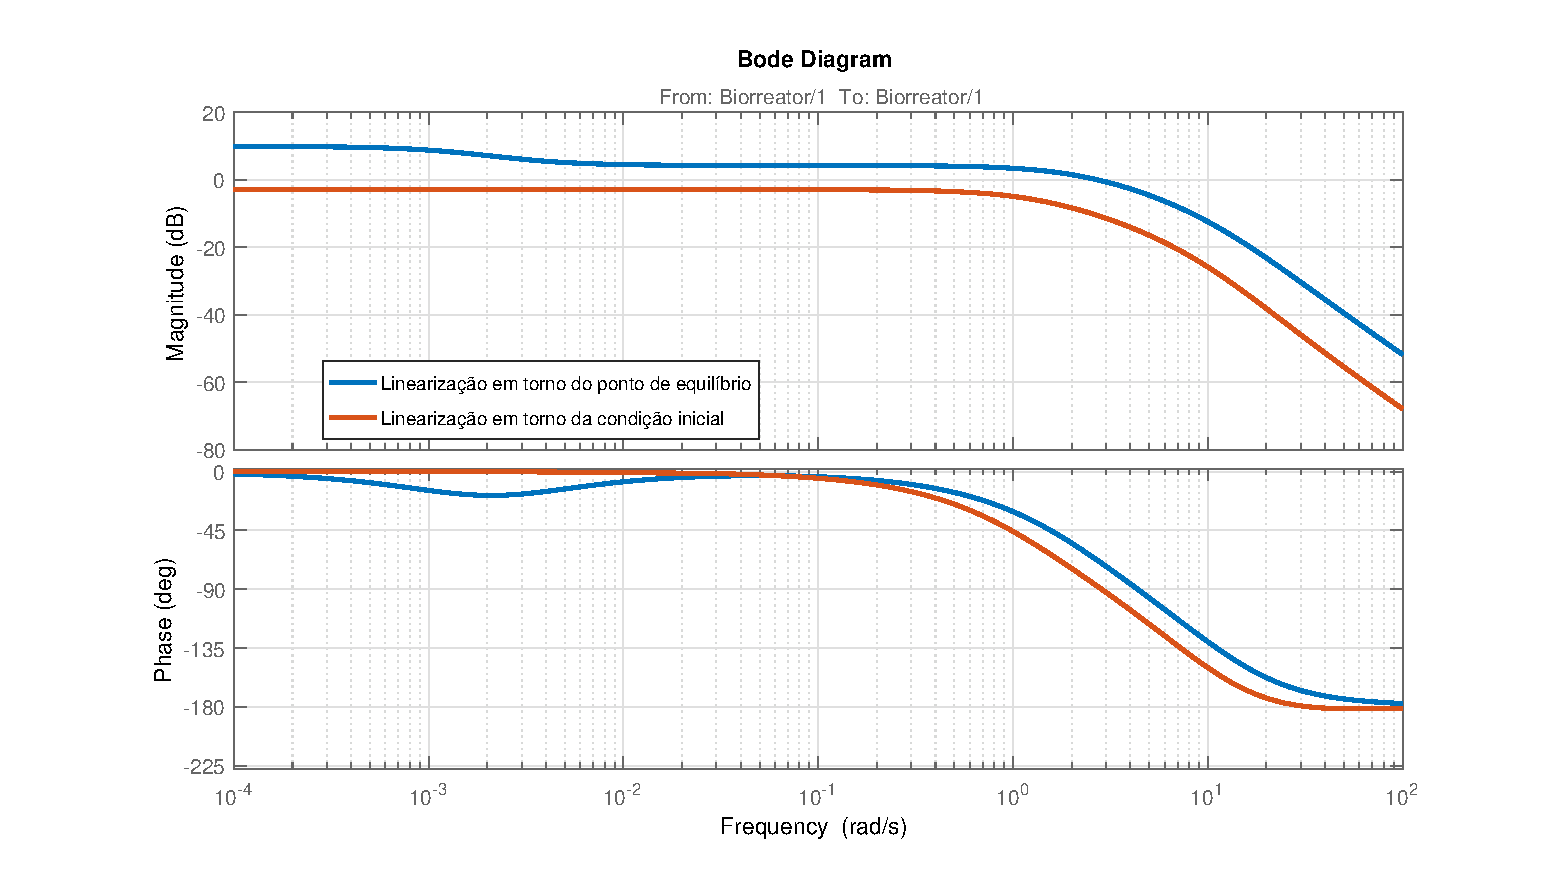
\includegraphics[width=1\textwidth]{figures/bode.eps}
\caption{Diagrama de bode dos modelos linearizados no instante inicial e no equilíbrio}
\end{figure}
\end{center}

\end{frame}

\section{Resultados}
\subsection{Resultados}
\begin{frame}[fragile]{Resultados}
\begin{tcolorbox}[title= Controlador]
\begin{gather}
S_{1in}(t) =  0.143 \cdot (r(t)-q_m(t)) + 1 \cdot \int_{0}^{t} r(\tau)-q_m(\tau) d\tau  \label{PI} \nonumber
\end{gather} 
\end{tcolorbox}
\end{frame}

\begin{frame}[fragile]{Resultados}
\begin{figure}
%comparação com o sistema em malha aberta
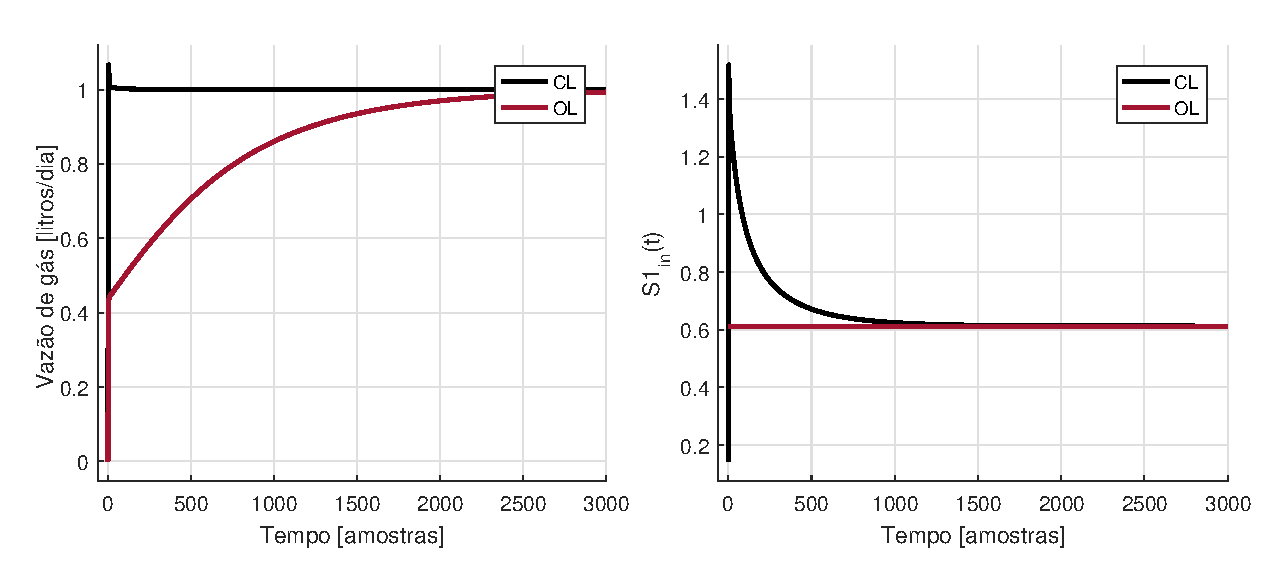
\includegraphics[width=1\textwidth]{figures/comparacao.eps}
\caption{Comparação entre o desempenho em simulação do sistema em malha aberta (OL) e em malha fechada (CL)}
\end{figure}
\end{frame}

\section{Conclusões}
\begin{frame}[fragile]{Conclusões}
O controlador PI proporcional significativa melhoria de desempenho em relacão ao sistema em MA. Além disso, provê robustez a perturbações externas e a pequenas variações paramétricas. A fim de aperfeiçoar os resultados obtidos, sera necessária a implementacão efetiva do controlador in situ.
\end{frame}





% \begin{frame}[fragile]{Resolução dos problemas matemáticos inerentes ao modelo}
% \metroset{block=fill}
% \begin{block}{Problema:}
% Minimize $J(\theta)\equiv \frac{1}{N} \sum_{k=1}^N (q_M(kT)-\hat{q}_{M}(kT,\theta))^2$, onde $\theta\equiv [\mu_{1} \, K_{S_{1}} \, \mu_{2} \, K_{S_{2}} \, k_1 \, k_2 \, k_3 \, k_6]$, $\hat{q}_{M}(kT,\theta)$ é a saída do modelo do biorreator, assumindo que os valores das constantes são aquelas do vetor $\theta$, e $N$ é o número de amostras disponíveis. 
% \end{block}
% \end{frame}

% \begin{frame}[fragile]{Resolução dos problemas matemáticos inerentes ao modelo}
% A resolução do problema se dá pela discretização da equação utilizando os métodos de Runge-Kutta e a pela estimação iterativa dos valores do vetor de parâmetros $\theta$, utilizando algoritmos como o \textit{simplex Nelder-Mead} e o \textit{Trust-Region-Reflective}.

%     %\begin{center}
%     %\begin{figure}[b]
%     %\includegraphics[width=0.8\textwidth]{rk2.png}+
%     % \caption{Representação do método de Runge-Kutta 2 \cite{gilat2009metodos}}
%     %\end{figure}
%     %\end{center}
    
% \end{frame}

% \section{Resultados}
% \begin{frame}[fragile]{Resultados}
% De acordo com ARTIGO DINCON ->(NAO ACHEI NO GOOGLE SCHOLAR PARA CITAR)<-, a implementação em Matlab do algoritmo Trust-Region-Reflective (função \textbf{lsqonlin}) proporciona menor custo computacional e uma melhor qualidade de resultados.

% \end{frame}

% \begin{frame}[fragile]{Resultados}
%     \begin{center}
%     \begin{figure}[b]
%     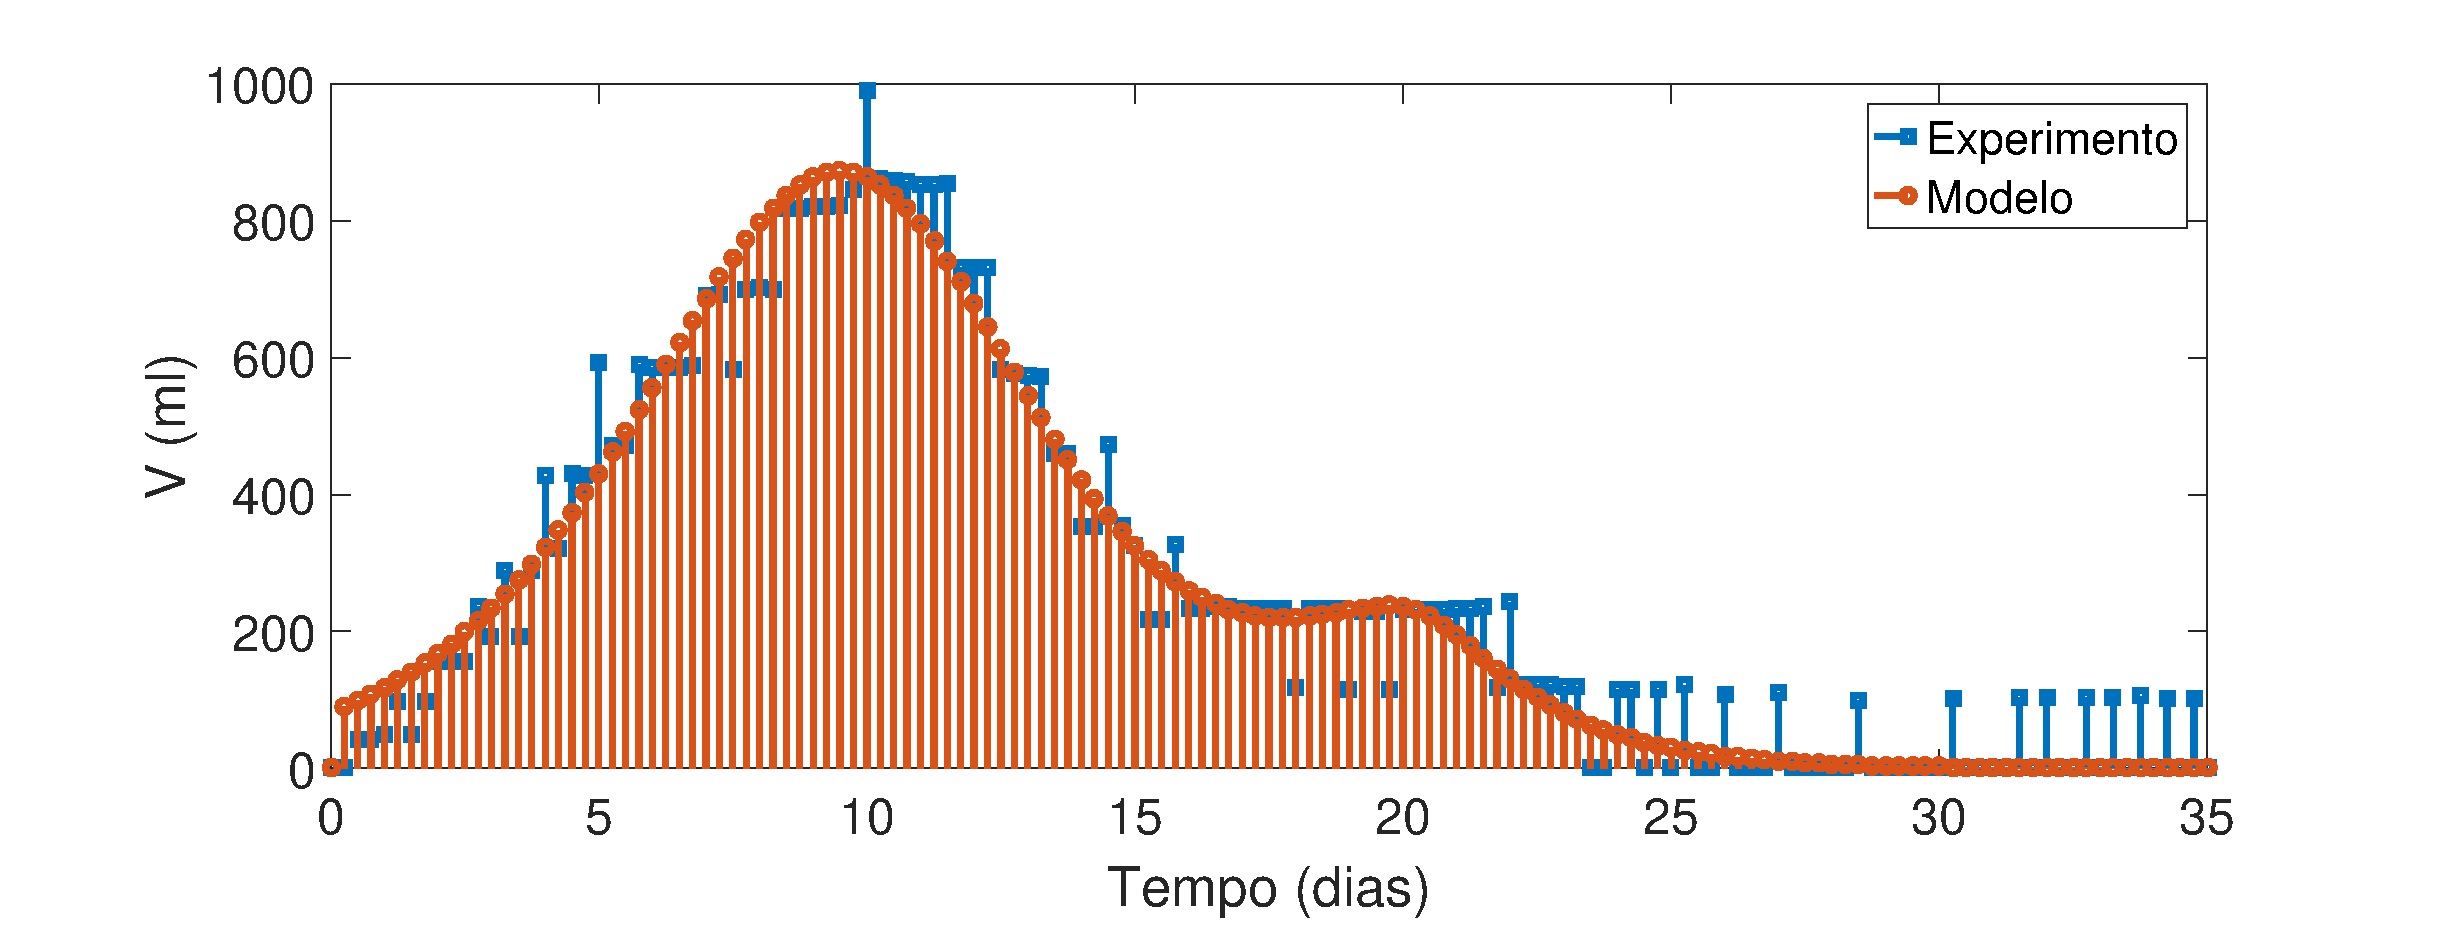
\includegraphics[width=1\textwidth]{simulacao.eps}+
%      \caption{Comparação entre a simulação numérica do modelo do biorreator e os dados reais}
%     \end{figure}
%      \end{center}    

% \end{frame}

% \begin{frame}[fragile]{Resultados}
%     \begin{center}
%     \begin{figure}[b]
%     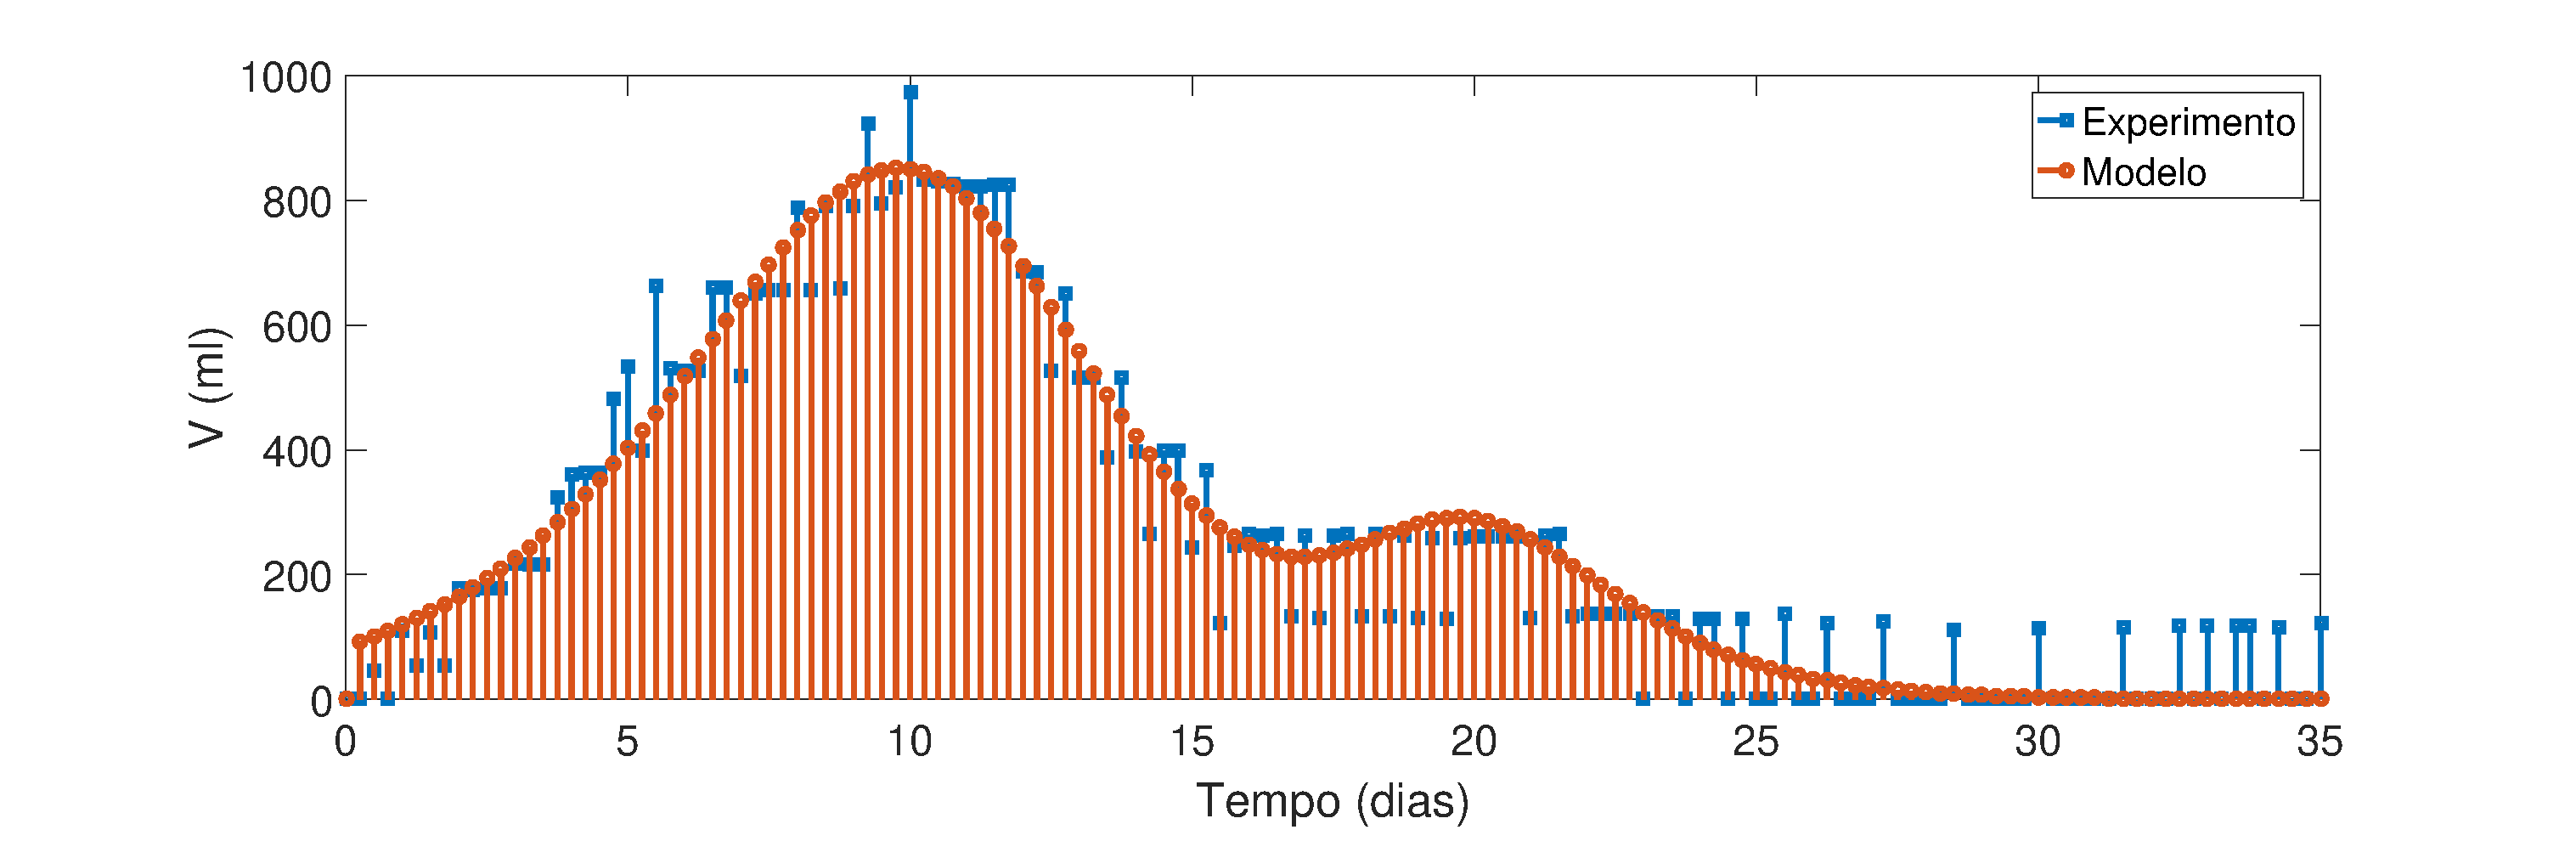
\includegraphics[width=1\textwidth]{simulacao2.eps}+
%      \caption{Comparação entre a simulação numérica do modelo do biorreator e os dados reais}
%     \end{figure}
%      \end{center}

% \end{frame}


% {%
% %\setbeamertemplate{frame footer}{My custom footer}
% %\begin{frame}[fragile]{Frame footer}
% %    \themename defines a custom beamer template to add a text to the footer. %It can be set via
% %    \begin{verbatim}\setbeamertemplate{frame footer}{My custom footer}%\end{verbatim}
% %\end{frame}
% %}

% \section{Conclusão}
% \begin{frame}[fragile]{Conclusão}
% 	Os resultados demonstram que o modelo de quatro estados utilizado é adequado ao processo que se deseja modelar. Dessa forma, poderemos utilizar esse modelo para projetarmos o controle de um processo baseado na inserção de matéria orgânica, com o intuito de maximizar a produção de gás metano.
% \end{frame}

% %\begin{frame}{Summary}

% %  Get the source of this theme and the demo presentation from

%  % \begin{center}\url{github.com/matze/mtheme}\end{center}

%   %The theme \emph{itself} is licensed under a
%   %\href{http://creativecommons.org/licenses/by-sa/4.0/}{Creative Commons
%   %Attribution-ShareAlike 4.0 International License}.

% %  \%begin{center}\ccbysa\end{center}

% %\end{frame}

\begin{frame}[allowframebreaks]{References}
   \bibliography{references}
   \bibliographystyle{abbrv}
   \nocite{alvarenga1977fundamentos}
\end{frame}

 \begin{frame}[standout]
   Perguntas?
 \end{frame}

% %\appendix

% %\begin{frame}[fragile]{Backup slides}
% %  Sometimes, it is useful to add slides at the end of your presentation to
% %  refer to during audience questions.

% %  The best way to do this is to include the \verb|appendixnumberbeamer|
% %  package in your preamble and call \verb|\appendix| before your backup slides.

% %  \themename will automatically turn off slide numbering and progress bars for
% %  slides in the appendix.
% %  \end{frame}

\end{document}
